\documentclass{book}

\usepackage{../Package/latexa}
\usepackage{../Package/algebra}
\usepackage{../Package/theorema}
\usepackage{../Package/diagramma}
\usepackage{../Package/categoria}

\usepackage{tikz}
\usepackage{tikz-cd}
\usetikzlibrary{arrows}

\newcommand{\qi}{\backsimeq_{\textsc{QI}}}
\newcommand{\ba}{\backsimeq_{\textsc{BA}}}
\newcommand{\normal}{\vartriangleleft}
\newcommand{\tm}{\subset}
\newcommand{\Stab}[2]{\textsf{Stab}_{#1}(#2)}
\newcommand{\Cay}[2]{\textsf{Cay}(#1,#2)}


\renewcommand{\A}{\mathbb{A}}

\renewcommand{\i}{^{-1}}

\newcommand{\af}{\mathfrak{a}}
\newcommand{\Af}{\mathfrak{A}}
\renewcommand{\bf}{\mathfrak{b}}
\newcommand{\Bf}{\mathfrak{B}}
\newcommand{\cf}{\mathfrak{c}}
\newcommand{\Cf}{\mathfrak{C}}
\newcommand{\ff}{\mathfrak{f}}
\newcommand{\Ff}{\mathfrak{F}}
\newcommand{\pf}{\mathfrak{p}}
\newcommand{\Pf}{\mathfrak{P}}
\newcommand{\mf}{\mathfrak{m}}
\newcommand{\Mf}{\mathfrak{M}}

\newcommand{\Frob}{\textsf{Frob}}

\newcommand{\Leg}[2]{\left(\frac{#1}{#2}\right)}

\begin{document}

\tableofcontents

\chapter{Topologische Gruppen}
\section{Topologische Gruppen}
\Def{Topologische Gruppen}
Ein Paar $(G,\T)$ einer Gruppe und einer Topologie auf $G$ heißt \df{topologische Gruppe}, wenn die Abbildungen
\begin{align*}
\_\cdot\_ : G \times G &\Pfeil{} G\\
\_\i : G &\Pfeil{} G
\end{align*}
stetig sind.\\
Unter einem \df{Homomorphismus topologischer Gruppen} verstehen wir einen stetigen Gruppenhomomorphismus.

\Bem{}
Seien $G,H$ topologische Gruppen.
\begin{itemize}
\item $U \subset G$ heißt \df{Umgebung} von $g\in G$, falls eine Teilmenge $V \subset_o G$ existiert, sodass $g \in V \subseteq U$.
\item $\phi: G \pfeil{} H$ ist genau ein Homomorphismus, wenn das Urbild jeder Umgebung der 1 in $H$ eine Umgebung der 1 in $G$ ist.
\end{itemize}

\Prop{}
\label{Prop4}
Sei $G$ eine topologische Gruppe und $U \subset G$ eine Umgebung der 1.
\begin{itemize}
\item[(i)] Es existiert eine offene Umgebung $V$ der 1, sodass $V\cdot V \subset U$ und $V = V\i$.
\item[(ii)] Es existiert eine Umgebung $V$ der 1, deren Abschluss $\overline{V}$ in $U$ enthalten ist.
\end{itemize}
Sei nun $H \leq G$ eine Untergruppe.
\begin{itemize}
\item[(iii)] Der Abschluss von $H$ ist ebenfalls eine Untergruppe. Dieser ist insbesondere normal, falls $H$ ebenfalls normal ist.
\item[(iv)] Ist $H \leq_o G$ offen, so auch abgeschlossen, also insbesondere eine Zusammenhangkomponente.
\end{itemize}
\begin{Beweis}{}
\begin{itemize}
\item[(i)] Definiere
\begin{align*}
f&: G \pfeil{} G, x \mapsto x^2\\
V' &:= f\i(U) \cap U\\
V &:= V' \cap {V'}\i
\end{align*}
\item[(ii)] Wir geben ohne Beweis einen Satz an, aus dem die Behauptung sofort folgt:
\paragraph{Satz von Weil}
Eine topologische Gruppe $G$ ist $\text{T}_{3\frac{1}{2}}$, d.\,h., ist $A\subseteq_aG$ eine Teilmenge, die die 1 nicht enthält, so existiert eine stetige Abbildung $f : G \pfeil{} [0,1] \subset \R$ mit folgenden Eigenschaften:
\begin{itemize}
\item $f(A) = \{1\}$
\item $f(1) = 0$
\end{itemize}
\item[(iii)] Seien $a,b \in \overline{H}$, dann existieren Folgen $a_n,b_n \in H$, die gegen $a,b$ konvergieren. Dann ist $(a_n,b_n\i)$ eine Folge in $G\times G$, die gegen $(a,b\i)$ konvergiert. Da Multiplikation stetig ist, konvergiert $a_nb_n\i \in H$ gegen $ab\i$, ergo liegt $ab\i$ in $\overline{H}$. Analog zeigt man, dass $\overline{H}$ normal ist, falls $H$ normal ist.
\item[(iv)] Sei $H \leq_o G$ offen und sei $a \in \overline{H}$. Dann existiert eine Folge $a_n \in H$, die gegen $a$ konvergiert. $aH$ ist eine Umgebung von $a$, ergo existiert ein $N \in \N$, sodass $a_n \in aH$. Daraus folgt $a \in a_nH\i = H$.
\end{itemize}
\end{Beweis}

\Prop{}
\label{Prop5}
Sei $G$ eine topologische Gruppe. Dann sind folgende Aussagen äquivalent:
\begin{itemize}
\item[(i)] $G$ ist hausdorffsch.
\item[(ii)] $\{1\}$ ist abgeschlossen in $G$.
\item[(iii)] $\{g\}$ ist abgeschlossen in $G$ für alle $g \in G$.
\end{itemize}
\begin{Beweis}{}
Es bleibt die Implikation (iii) $\Impl{}$ (i) zu zeigen. Seien $g,h \in G$ verschieden. Dann ist $U = G \setminus \{gh\i\}$ offen in $G$. Laut Proposition \ref{Prop4} (i) existiert eine offene Teilmenge $V$ von $U$ mit folgenden Eigenschaften:
\begin{itemize}
\item $1\in V$
\item $VV \subset U$
\item $V\i = V$
\end{itemize}
Dann sind $Vg, Vh$ disjunkte Umgebungen von $g,h$. Denn wäre ihr Schnitt nichtleer, so würden $v,w\in V$ existieren, sodass $vg  = wh$, woraus folgt dass $gh\i $ in $ U$ liegen würde.
\end{Beweis}

\Prop{}
\label{Prop6}
Sei $G$ eine topologische Gruppe und $H \leq G$ eine Untergruppe.
\begin{itemize}
\item[(i)] $H$ ist genau dann diskret, wenn $H$ einen isolierten Punkt besitzt.
\item[(ii)] Ist $G$ hausdorffsch und $H$ diskret, so ist $H$ abgeschlossen.
\end{itemize}
\begin{Beweis}{(ii)}
$H$ ist diskret, d.\,h., es existiert eine offene Teilmenge $V \subseteq_o G$, s.\,d. $V \cap H = \{1\}$. Ohne Einschränkung darf angenommen werden, dass $V = V\i$.\\
G ist hausdorffsch, ergo ist $\{1\}$ abgeschlossen in $V$. Sei $x \in \overline{H}$, dann existiert ein $y \in H$, das in $xV$ liegt. Man erhält durch Umformung
\[ x \in yV \cap \overline{H} = \bigcap_{H \subset A \subset_a G} A \cap yV = \bigcap_{\{y\} = H \cap yV \subset A \subset_a yV} A  = \{y\} \]
Ergo gilt $x = y \in H$.
\end{Beweis}

\Prop{}
\label{Prop1.1.8}
Sei $G$ eine topologische Gruppe mit Untergruppe $H$.
\begin{itemize}
\item $G$ operiert stetig auf $G/H$.
\item $\pi_H : G \pfeil{} G/H$ ist eine offene Abbildung.
\item $G/H$ ist genau dann hausdorffsch, wenn $H$ abgeschlossen ist.
\item $G/H$ ist genau dann diskret, wenn $H$ offen ist.
\item Ist $H$ normal, so ist $G/H$ eine topologische Gruppe und $\pi_H$ ein Morphismus topologischer Gruppen.
\end{itemize}
\begin{Beweis}{(iii)}
 $\Longrightarrow$: Sei $a \in \overline{H}$, dann existiert eine Folge $a_n \in H$, die gegen $a$ konvergiert. Da $\pi_H$ stetig ist, gilt
\[ \pi_H(a_n) \Pfeil{n\pfeil{} \infty} \pi_H(a) \]
Da alle $a_n$ in $H$ liegen, gilt aber $\pi_H(a_n) = \pi_H(1)$. Da $G/H$ hausdorffsch ist, besitzt diese Folge höchstens einen Grenzwert, ergo gilt
\[ \pi_H(a) = \pi_H(1) \Impl{} a \in H \]
$\Longleftarrow$: Seien $\pi_H(b),\pi_H(c) \in G/H$. Ohne Einschränkung nehmen wir an, dass $\pi_H(c) = \pi_H(1)$.\\
In jeder Umgebung $\widetilde{U}$ von $\pi_H(b)$ sei $\pi_H(1)$ enthalten. Dann ist $b$ im Abschluss von $H$ enthalten, denn ist $U$ eine Umgebung von $b$, so ist $\pi(U)_H$ eine Umgebung von $\pi_H(b)$. Ergo ist $\pi_H(1) \in \pi_H(U)$, ergo existiert ein $h \in H$, sodass $h \in U$.
\end{Beweis}

\Def{}
Ist $G$ eine topologische, so ist $\overline{\{1\}}$ normal. $G/\overline{\{1\}}$ wird als \df{Hausdorffquotient} von $G$ bezeichnet.

\Def{}
Ein Homomorphismus $\phi : G \pfeil{} G'$ topologischer Gruppen heißt \df{strikt}, falls er den Isomorphiesatz respektiert, d.\,h., die induzierte Abbildung
\[ \phi : G / \Ker \phi \Pfeil{} \Img \phi \]
ist homöomorph.

\Def{}
Eine kurze exakte Sequenz topologischer Gruppen heißt \df{topologisch exakt}, falls alle beteiligten Abbildungen strikt sind.

\section{Lokal-Kompakte Gruppen}
\Def{}
Sei $X$ ein topologischer Raum.
\begin{itemize}
\item Wir nennen $X$ \df{kompakt}, falls er \df{quasikompakt} ist, d.\,h., jede offene Überdeckung von $X$ besitzt eine offene Teilüberdeckung.
\item $X$ heißt \df{lokal kompakt}, falls jeder Punkt eine Umgebung enthält, deren Abschluss kompakt ist.
\end{itemize}

\Bem{}
\begin{itemize}
\item Jede abgeschlossene Teilmenge eines kompakten Raumes ist kompakt.
\item Jede kompakte Menge eines Hausdorffraums ist abgeschlossen.
\item Ist ein Raum kompakt und hausdorffsch, so erfüllt er \df{T3}, d.\,h., er ist \df{regulär}, d.\,h., jede abgeschlossene Teilmenge und jeder nicht in dieser Teilmenge liegender Punkt könne durch offene Umgebungen getrennt werden.
\item Ein Raum ist genau dann regulär, wenn jeder Punkt eine Umgebungsbasis aus abgeschlossenen Umgebungen besitzt.
\item In lokal kompakten Räumen hat jeder Punkt eine Umgebungsbasis aus kompakten Umgebungen.
\item Ist ein Raum kompakt und hausdorffsch, so erfüllt er \df{T4}, d.\,h., er ist \df{normal}, d.\,h., disjunkte abgeschlossene Teilmengen werden durch offene Umgebungen getrennt.
\item Eine bijektive, stetige Abbildung von einem Kompaktum nach einem Hausdorffraum ist homöomorph.
\end{itemize}

\Prop{}
Sei $G$ eine lokal kompakte Gruppe, $H\leq G$ eine abgeschlossene Gruppe.
\begin{itemize}
\item $G/H$ ist ein lokal kompakter Raum.
\item Jede kompakte Teilmenge von $G/H$ besitzt ein kompaktes Urbild.
\end{itemize}

\Prop{}
Sei $G$ lokal kompakt und hausdorffsch, $H \leq G$ eine Untergruppe.\\
$H$ ist genau dann diskret, wenn $H\cap K$ für alle kompakten Teilmengen von $K \subset G$ endlich ist.

\section{Zusammenhangkomponenten}
\Def{}
Ein topologischer Raum heißt \df{zusammenhängend}, wenn er sich nicht in zwei offene, disjunkte, nichtleere Teilräume zerlegen lässt.

\Bem{}
\begin{itemize}
\item Ist eine Teilmenge eines Raumes zusammenhängend, so ist es auch ihr Abschluss.
\item Seien $A_i \subset X$ jeweils zusammenhängend, dann gilt
\[ \bigcap_{i\in I}A_i \neq \emptyset \Impl{} \bigcup_{i\in I} A_i \text{ ist zusammenhängend} \]
\item Beliebige Produkte zusammenhängender Räume sind zusammenhängend.
\item Bilder zusammenhängender Räume bleiben unter stetigen Abbildungen zusammenhängend.
\end{itemize}

\Def{}
Sei $X$ ein topologischer Raum.
\begin{itemize}
\item Ist $x \in X$ ein Punkt, so verstehen wir unter der \df{Zusammenhangkomponente} von $x$ die größte, zusammenhängende Teilmenge von $X$, die $x$ enthält.
\item $X$ heißt \df{total unzusammenhängend}, wenn jede Zusammenhangkomponente genau ein Element enthält.
\item Ist $G$ eine topologische Gruppe, so bezeichnen wir mit $G^o$ die Zusammenhangkomponente der Eins. 
\end{itemize}

\Prop{}
Ist $G$ eine topologische Gruppe, so ist $G^o$ ein abgeschlossener Normalteiler.

\Prop{}
Sei $G$ eine topologische Gruppe, $H \leq G$ eine Untergruppe. Sind $H$ und $G/H$ zusammenhängend, so auch $G$.

\Prop{}
Sei $G$ eine topologische Gruppe, dann ist $G/G^o$ hausdorffsch und total unzusammenhängend.

\Bem{}
Eine total unzusammenhängende Gruppe ist hausdorffsch.

\section{Total Unzusammenhängende Gruppen}
\Satz{}
Eine hausdorffsche Gruppe ist genau dann total unzusammenhängend und lokal kompakt, wenn jede Umgebung der Eins eine offene und kompakte Untergruppe enthält.

\Lem{}
Sei $X$ ein kompakter und total unzusammenhängender Hausdorffraum. Bezeichnet $\mathcal{W}$ für $x \in X$ die Menge der Umgebungen von $x$, die zugleich offen und abgeschlossen sind, so gilt
\[ \bigcap_{W\in \mathcal{W}} W = \{x\} \]

\Lem{}
Sei $G$ eine lokal kompakte und total unzusammenhängende Gruppe, $U$ eine offene Umgebung von $x \in G$.\\
Dann existiert eine offene und kompakte Umgebung von $x$, die in $U$ enthalten ist.

\Kor{}
Sei $G$ eine kompakte und total unzusammenhängende Gruppe. Dann enthält jede Umgebung der Eins einen offenen Normalteiler.

\section{Limiten Topologischer Räume}
\Def{Gerichtet Geordnet}
Sei $I$ eine nichtleere Menge.
\begin{itemize}
	\item $(I,\leq)$ heißt \df{teilgeordnet}, falls $\leq$ auf $I$ eine binäre Relation ist, die reflexiv und transitiv ist.
	\item Eine teilgeordnete Menge $(I,\leq)$ heißt \df{gerichtet}, falls für jedes Paar $i,j \in I$ ein $k \in I$ existiert, sodass $i \leq k$ und $j\leq k$.
\end{itemize}

\Def{Inverses System}
Sei $I$ gerichtet.
\begin{itemize}
	\item Ein \df{inverses System} $(X_i, \phi_{ij})$ topologischer Räume ist ein kontravarianter Funktor $X : I \pfeil{} \Top$, d.\,h., die $X_i$ sind topologische Räume und für jedes $i\leq j$ ist
	\[\phi_{ij} :X_j \Pfeil{}X_i \]
	eine stetige Abbildung.
	\item Ein Morphismus inverser Systeme ist eine natürliche Transformation von inversen Systemen.
	\item Ist $X$ ein topologische Raum, so verstehen wir unter $(X, \id{X})$ das \df{konstante System} zu $X$.
\end{itemize}

\Def{Projektiver Limes}
Ein \df{projektiver bzw. inverser Limes} eines inversen Systemes $(X_i, \phi_{ij})$ ist ein topologischer Raum
\[ X = \lim\limits_{i \in I}(X_i, \phi_{ij}) =: \lim\limits_{i\in I}X_i \]
der den Funktor
\begin{align*}
\Top &\Pfeil{} \textbf{Set}\\
Y & \longmapsto \Hom{\text{inv.Sys.}}{(Y,\id{Y})}{(X_i, \phi_{ij})}
\end{align*}
darstellt, d.\,h.,
\[ \Hom{\Top}{Y}{X}  \isom{} \Hom{\text{inv.Sys.}}{(Y,\id{Y})}{(X_i, \phi_{ij})} \]

\Bem{}
\begin{itemize}
	\item Ein Limes ist eindeutig bis auf eindeutige Isomorphie.
	\item Folgendes Konstrukt ist ein Limes von $(X_i, \phi_{ij})$
	\[ X:= \set{(x_k) \in \prod_{i\in I}X_i }{ \phi_{ij}(x_i) = x_j \forall i \leq j } \]
	\item Es gilt
	\[ X= \bigcap_{i\leq j} \set{(x_k) \in \prod_{i\in I}X_i }{ \phi_{ij}(x_i) = x_j} \]
\end{itemize}

\Prop{}
Sei $(X_i, \phi_{ij})$ ein inverses System topologischer Räume mit stetigen Abbildungen
\[ \phi_i : X_i \Pfeil{} X:= \lim\limits_{i \in I} X_i \]
\begin{itemize}
	\item Die $\phi_i\i$ bilden für alle $i$ und $U\subseteq_o X_i$ eine Basis der Topologie von $X$.
	\item Eine Teilmenge $Y \subset X$ mit $\phi_i(Y) = X_i$ für alle $i\in I$ liegt dicht in $X$.
	\item Eine Abbildung $f : X \pfeil{} Y$ ist genau dann stetig, wenn für alle $i \in I$ $\phi_i\circ f$ stetig ist.
\end{itemize}
\Prop{}
Sei $(X_i,\phi_{ij})$ ein inverses System topologischer Räume mit Limes $X$.
\begin{itemize}
	\item Sind alle $X_i$ hausdorffsch, so ist dies auch $X$.
	\item Sind alle $X_i$ total unzusammenhängend, so auch $X$.
	\item Sind alle $X_i$ hausdorffsch, so ist
	\[\set{(x_k) \in \prod_{i\in I}X_i }{ \phi_{ij}(x_i) = x_j \forall i \leq j }\]
	eine abgeschlossene Teilmenge von $\prod_{i \in I}X_i$.
	\item Sind alle $X_i$ kompakt und hausdorffsch, so ist es auch $X$.
	\item Sind alle $X_i$ nichtleer, kompakt und hausdorffsch, so ist dies auch $X$.
\end{itemize}
\Prop{}
Seien folgende Morphismen inverser Systeme von kompakten und hausdorffschen Gruppen gegeben
\begin{align*}
 (F_i, \upsilon_{ij}) \Pfeil{\alpha} (G_i, \phi_{ij}) \Pfeil{\beta} (H_i, \chi_{ij})
\end{align*}
Ist diese Sequenz gradweise exakt, d.\,h., ist für alle $i \in I$
\[ F_i \Pfeil{\alpha_i} G_i \Pfeil{\beta_i} H_i \]
exakt, so ist auch die Limessequenz
\[ \lim\limits_{i\in I} F_i \Pfeil{\alpha} \lim\limits_{i \in I}G_i \Pfeil{\beta} \lim\limits_{i \in I}H_i \]
exakt.

\Def{Kolimes}
Sei $I$ gerichtet.
\begin{itemize}
	\item Ein \df{direktes System} topologischer Räume ist ein kovarianter Funktor
	\[X : I \Pfeil{} \Top\]
	\item Morphismen direkter System sind natürliche Transformationen der zugrunde liegenden Funktoren.
	\item Ein \df{Kolimes} eines direkten Systemes $(X_i, \phi_{ij})$ ist ein topologischer Raum $X = \textsf{colim}_{i\in I}X_i$, der den Funktor
	\[ Y \longmapsto \Hom{}{(X_i,\phi_{ij})}{(Y,\id{Y})} \]
	darstellt.
\end{itemize}

\Bem{}
Ist $(X_i,\phi_{ij})$ ein direktes System, so ist folgender Kolimes gegeben
\[ \coprod_{i\in I}X_i/\sim \]
wobei
\[ x_i \sim x_j \Gdw{} \exists k \geq i,j : \phi_{ik}(x_i) = \phi_{jk}(x_j) \]

\section{Proendliche Gruppe}
\Bem{}
Jede endliche Gruppe wird als eine topologische Gruppe aufgefasst, indem wir sie mit der diskreten Topologie versehen.
\Def{}
Eine topologische Gruppe heißt \df{proendlich}, wenn sie ein projektiver Limes eines inversen Systems endlicher Gruppen ist.
\Satz{}
Sei $G$ eine topologische Gruppe. Folgende Aussagen sind äquivalent:
\begin{itemize}
	\item $G$ ist proendlich.
	\item $G$ ist kompakt und total unzusammenhängend.
	\item $G$ ist kompakt und
	\[ \bigcap_{N\trianglelefteq_o G}N = \{1\} \]
\end{itemize}

\Lem{}
Sei $G$ eine topologische Gruppe, $I$ eine Familie abgeschlossener Normalteiler, sodass gilt
\[ N_1,N_2 \in I \Impl{} \exists N_3 \in I: N_3 \subseteq N_1 \cap N_2 \]
\begin{itemize}
	\item Definiere für $N_1,N_2\in I$
	\[ N_1\preceq N_2 \Gdw{} N_1 \supseteq N_2 \]
	Dann ist $(I,\preceq)$ gerichtet.
	\item Setzt man für $N_i \preceq N_j$
	\[ \phi_{ij} : G/N_j \Pfeil{} G/N_i \]
	so ist $(G/N_i, \phi_{ij})$ ein inverses System.\\
	Definiere
	\[ \widehat{G} := \lim\limits_{N \in I}G/N \]
	Es existiert ein kanonischer Morphismus stetiger Gruppen
	\[ \upsilon : G \Pfeil{} \widehat{G} \]
	mit Kern
	\[\Ker \upsilon = \bigcap_{N\in I}N \]
	\item Ist $G$ kompakt, so ist $\upsilon$ surjektiv.
\end{itemize}

\section{Unendliche Galoistheorie}

\Satz{}
Sei $L|K$ eine galoissche, nicht notwendigerweise endliche Körpererweiterung. Definiere
\[ G(L|K) :=\Aut{K-\text{Alg.}}{L} \]
$G(L|K)$ erhält eine Topologie als Gruppe, indem wir Untergruppen der Gestalt
\[ G(L|E) \]
für alle endlichen, galoisschen Teilerweiterungen $E|K$ zu einer Umgebungsbasis der Eins in $G(L|K)$ zusammenfassen. Es gilt dann
\[ G = \lim\limits_{\stackrel{L|E|K}{E|K \text{ endl., gal.}}}G(E|K) \]

\Satz{Satz der Unendlichen Galoistheorie}
Für eine galoissche Körpererweiterung  $K$ herrschen folgende Dualitäten vor
\begin{center}
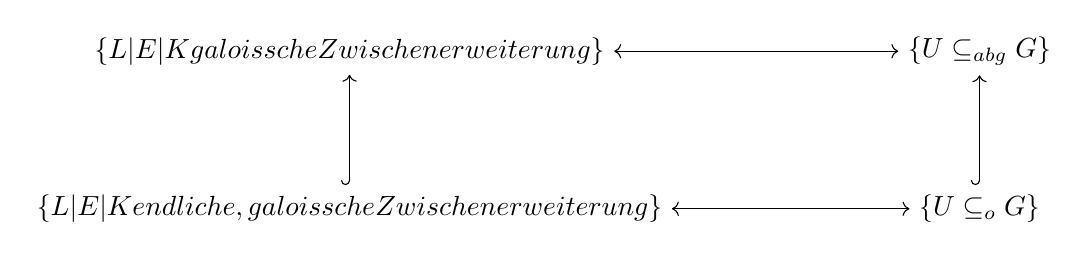
\begin{tikzpicture}[scale =2]
\node (D1) at (0,1)  {$\{L|E|K\text{ galoissche Zwischenerweiterung}\}$};
\node (D3) at (4,1)  {$\{ U \subseteq_\text{abg} G \}$};
\node (D5) at (4,0)  {$\{U \subseteq_o G \}$};
\node (D7) at (0,0)  {$\{L|E|K\text{endliche, galoissche Zwischenerweiterung}\}$};

\draw[<->] (D1) -> (D3);
\draw[<->] (D5) -> (D7);
\draw[right hook->] (D5) -> (D3);
\draw[right hook->] (D7) -> (D1);
%\draw [ultra thick, right hook->,    blue] (0,-1) -- (3,-1);
\end{tikzpicture}
\end{center}
durch
\begin{align*}
E & \longmapsto G(L|E)\\
H & \longmapsto L^H
\end{align*}



\chapter{Klassenkörpertheorie -- Motivation und Hauptresultate}
\section{Abelsche Erweiterungen von $\Q$}
\Satz{Kroncker-Weber}
Sei $L|\Q$ eine endliche Erweiterung. Folgende Aussagen sind äquivalent:
\begin{itemize}
	\item $L|\Q$ ist abelsch.
	\item $L$ ist enthalten in einem Kreisteilungskörper $\Q(\mu_n)$.
\end{itemize}

\Satz{}
Sei $N \in \N$, $L |\Q$ endlich. Folgende Aussagen sind äquivalent:
\begin{itemize}
	\item $L \subseteq \Q(\mu_N)$.
	\item Ob eine Primzahl $p$ in $L$ voll zerlegt ist, hängt nur von $p\mod{n}$ ab.
\end{itemize}

\Satz{}
Sei $L|\Q$ abelsch und $N$ minimal mit
\[ L \subseteq \Q(\mu_N) \]
Für jede Primzahl $p$ gilt
\[ p \text{ ist in }L \text{ verzweigt} \Gdw{} p|N \]

\Satz{}
Sei $N \in \N$ und $H \subseteq (\Z/N\Z)^\times \isom{} G(\Q(\mu_N) / \Q)$ beliebig. Es bezeichne $L = \Q(\mu_N)^H$.\\
Für $p\not | N$ prim gilt:
\begin{itemize}
	\item $p$ ist unverzweigt in $L$.
	\item $p$ ist genau dann voll zerlegt in $L$, wenn $p\mod{N} \in H$.
	\item Ist $f$ die kleinste natürliche Zahl, die
	\[ p^f \mod{N} \in H \]
	erfüllt, so ist $p\O_L$ ein Produkt von $[L:\Q]/f$ verschiedenen Primidealen. 
\end{itemize}

\Prop{}
Sei $L|K$ galoissch und $\Pf|\pf$ unverzweigte Stellen in $\O_L|\O_K$. Es bezeichne $\lambda = \O_L / \Pf$ und $\kappa = \O_K /\pf$ die korrespondierenden Restklassenkörper. Dann ist $G_\Pf := G(\lambda | \kappa) \inj{\iota} G(L|K)$ zyklisch und wird vom \df{Frobeniusautomorphismus}
\begin{align*}
\phi_q : \lambda & \Pfeil{} \lambda\\
x &\longmapsto x^q 
\end{align*}
erzeugt, wobei $q = \# \kappa$. Definiere für $\sigma \in G(L|K)$
\[ \Frob_{\pf, \Pf} := \iota(\phi_q) \text{ und } \Frob_{\pf, \sigma(\Pf)} := \sigma \Frob_{\pf, \Pf} \sigma\i \]
und folgende Äquivalenzklasse
\[ \Frob_\pf :=\Frob_{\pf,L} := \set{ \Frob_{\pf, \sigma(\Pf)} }{\sigma \in G(L|K)} \subset G(L|K) \]
Dann gilt
\begin{itemize}
	\item Es gilt $\Frob_\pf = \{1\}$ genau dann, wenn $\pf$ total zerlegt in $L|K$ ist.
	\item Es gilt
	\[ \#\{ \Pf' | \pf \} = \frac{\#G(L|K)}{\#G_{\Pf'}} \]
	\item Ist $L|K$ abelsch, so besteht $\Frob_\pf$ aus dem eindeutig bestimmten Element, das auf $\lambda$ die Abbildung $x \mapsto x^q$ induziert.
	\item Ist $L'|K$ eine galoissche Zwischenerweiterung, so gilt
	\[ \Frob_{\pf, L} \surj{res} \Frob_{\pf,L'} \]
\end{itemize}

\Prop{}
Es gelte $p\nmid N$. Dann ist $p$ unverzweigt in $\Q(\mu_N)$ und es herrscht folgende Isomorphie vor
\begin{align*}
\chi_{cyc, N} : G(\Q(\mu_N) | \Q) & \Pfeil{\isom{}} (\Z/NZ)^\times\\
\Frob_p & \longmapsto p \mod{N}
\end{align*}

\section{Quadratische Erweiterungen}
\Prop{}
Sei $m$ eine quadratfreie ganze Zahl. Dann ist $\Q(\sqrt{m}) | \Q$ abelsch. Setzt man
\begin{align*}
N := 
\left\lbrace\begin{aligned}
\bet{m} && m \equiv 1 \mod{4}\\
4\bet{m} && m \equiv 2,3 \mod{4}
\end{aligned}\right.
\end{align*}
so ist $N$ minimal mit der Eigenschaft
\[ \Q(\sqrt{m}) \subset \Q(\mu_N) \]

\Def{Legendre-Symbol}
Sei $p> 2$ eine ungerade Primzahl und $a \in \Z$ beliebig. Definiere das \df{Legendre-Symbol} durch
\[ \Leg{a}{p} := \left\lbrace 
\begin{aligned}
1 && p \nmid a \text{ und } a \in (\Z/p\Z^\times)^2\\
0 && p \mid a\\
-1 && p \nmid a \text{ und } a \notin (\Z/p\Z^\times)^2
\end{aligned}
\right. \]
wobei $(\Z/p\Z^\times)^2 = \set{x^2}{0\neq x \in \Z/p\Z}$ die Quadratzahlen modulo $p$ bezeichnet.\\
Die Abbildung $\Leg{\cdot}{p} : \Z/p\Z^\times \pfeil{} \{\pm 1\}$ ist multiplikativ, weswegen folgende kurze exakte Sequenz vorliegt
\[ 1 \Pfeil{} (\Z/p\Z^\times)^2 \Inj{} \Z/p\Z \Pfeil{\Leg{\cdot}{p}} \{\pm 1\} \Pfeil{} 1  \]
Ferner gilt
\[ \Leg{a}{p} = a^{\frac{p-1}{2}} \mod{p} \]

\Prop{Trivialer Zerlegungssatz}
Sei $m$ quadratfrei und $p$ eine ungerade Primzahl, die teilerfremd zu $p$ ist. Es gilt
\[ p\text{ ist voll zerlegt in }\Q(\sqrt{m}) \Gdw{} \Leg{m}{p} = 1 \]

\Def{Dirichlet-Charaktere}
Sei $m$ quadratfrei. Setze
\begin{align*}
N := 
\left\lbrace\begin{aligned}
\bet{m} && m \equiv 1 \mod{4}\\
4\bet{m} && m \equiv 2,3 \mod{4}
\end{aligned}\right.
\end{align*}
\begin{itemize}
\item Unter einem \df{Dirichlet-Charakter} verstehen wir einen Gruppenhomomorphismus
\[ \chi : (\Z / m\Z)^\times \Pfeil{} \C^\times \]
\item Ein Dirichlet-Charakter $\chi$ heißt \df{primitiv}, falls es kein $d \in \{1,\ldots, m-1\}$ gibt, für welches $\chi$ über
\[ (\Z / m\Z)^\times \Pfeil{}(\Z / d\Z)^\times \Pfeil{} \C^\times \]
faktorisiert.
\item Definiere
\begin{align*}
\chi_m : (\Z /N\Z)^\times  & \Pfeil{} \{\pm 1\} \subset \C^\times\\
a & \longmapsto \Theta_m(a) \cdot \prod_{\stackrel{e|m}{e > 2 \text{ prim}}}\Leg{a}{e} 
\end{align*}
wobei
\begin{align*}
\Theta_m(a) := \left\lbrace
\begin{aligned}
1 && m \equiv 1 \mod{4}\\
1 && m \equiv 3 \mod{4} \text{ und } a \equiv 1 \mod{4}\\
-1 && m \equiv 3 \mod{4} \text{ und } a \not\equiv 1 \mod{4}\\
1 && m \equiv 2 \mod{4} \text{ und } a \equiv 1 \text{ oder } 1 - m \mod{4}\\
-1 && m \equiv 2 \mod{4} \text{ und } a \not\equiv 1 \text{ oder } 1 - m \mod{4}
\end{aligned}
\right.
\end{align*}
\end{itemize}

\Lem{}
Sei $m$ quadratfrei. Setze
\begin{align*}
N := 
\left\lbrace\begin{aligned}
\bet{m} && m \equiv 1 \mod{4}\\
4\bet{m} && m \equiv 2,3 \mod{4}
\end{aligned}\right.
\end{align*}
Dann gilt
\begin{itemize}
\item $\chi_m$ ist primitiv.
\item 
\[ \chi_m(-1) = \left\lbrace
\begin{aligned}
1 && m > 0\\
-1 && m < 0
\end{aligned}
\right. \]
\end{itemize}

\Def{Gaußsche Summen}
Sei $\chi : (\Z/N\Z)^\times \pfeil{} \C^\times$ ein Dirichlet-Charakter und $\zeta_N$ eine primitive $N$-te Einheitswurzel. Definiere die \df{Gaußsche Summe} von $\chi$ und $\zeta_N$ durch
\[ G(\chi, \zeta_N) := \sum_{a \in \Z/N\Z^\times} \chi(a) \zeta_N^a \]
Bezeichne mit $\overline{\chi}$ den komplex konjugierten Charakter von $\chi$.

\Satz{}
Sei $\chi$ primitiv. Dann gilt
\begin{itemize}
\item Für alle $n \in \Z$ gilt
\[G(\chi, \zeta_N^n) = \overline{\chi}(n) G(\chi, \zeta_N) \]
\item $\bet{G(\chi, \zeta_N)} = \sqrt{N}$
\item Ist $m$ quadratfrei und gilt für $N$
\begin{align*}
N = 
\left\lbrace\begin{aligned}
\bet{m} && m \equiv 1 \mod{4}\\
4\bet{m} && m \equiv 2,3 \mod{4}
\end{aligned}\right.
\end{align*}
dann folgt
\[ G(\chi_m, \zeta_N)^2 = \left\lbrace
\begin{aligned}
m && m \equiv 1 \mod{4}\\
4m && m \equiv 2,3 \mod{4}
\end{aligned}
\right. \]
\end{itemize}

\Satz{}
Sei $m$ quadratfrei und $N = 
\left\lbrace\begin{aligned}
\bet{m} && m \equiv 1 \mod{4}\\
4\bet{m} && m \equiv 2,3 \mod{4}
\end{aligned}\right.$. \ Dann kommutiert folgendes Diagramm
\begin{center}
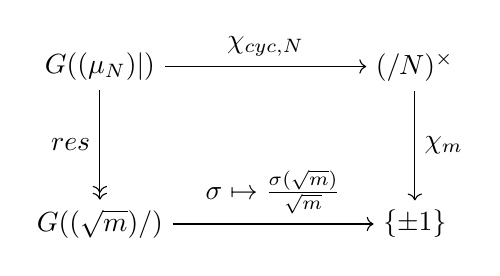
\begin{tikzpicture}[scale =1]
\node (D1) at (0,2)  {$G(\Q(\mu_N) | \Q)$};
\node (D3) at (4,2)  {$(\Z/N\Z)^\times$};
\node (D5) at (0,0)  {$G(\Q(\sqrt{m}) / \Q)$};
\node (D7) at (4,0)  {$\{\pm 1\}$};

\draw[->] (D1) -> (D3) node[midway, above]{$\isom{\chi_{cyc,N}}$};
\draw[->] (D5) -> (D7) node[midway, above]{$\sigma \mapsto \frac{\sigma(\sqrt{m})}{\sqrt{m}}$};
\draw[->] (D3) -> (D7) node[midway, right]{$\chi_m$};
\draw[->>] (D1) -> (D5) node[midway, left]{$res$};
%\draw [ultra thick, right hook->,    blue] (0,-1) -- (3,-1);
\end{tikzpicture}
\end{center}

\Satz{}
Sei $m$ quadratfrei und $N = 
\left\lbrace\begin{aligned}
\bet{m} && m \equiv 1 \mod{4}\\
4\bet{m} && m \equiv 2,3 \mod{4}
\end{aligned}\right.$\\
$p$ sei eine zu $N$ teilerfremde Primzahl. Es gilt
\[ p \text{ ist voll zerlegt in } \Q(\sqrt{m}) \Gdw{} \chi_m(p) = 1 \]

\Satz{Gaußsches Quadratisches Reziprozitätsgesetz}
Für zwei ungerade, verschiedene Primzahlen $p,q$ gilt
\[ \Leg{q}{p} = (-1)^{\frac{q-1}{2} \cdot \frac{p-1}{2} } \Leg{p}{q} \]

\paragraph{Ergänzungssätze}
\[ \Leg{-1}{p} = (-1)^{\frac{p-1}{2}} \text{ und } \Leg{2}{p} = (-1)^{\frac{p^2-1}{8}} \]

\Def{}
Sei $K$ ein Zahlkörper. Ein Element $a \in K^\times$ heißt \df{total positiv}, falls für alle reellen Stellen $\iota : K \inj{} \R$ gilt
\[ \iota(a) > 0 \]

\Satz{Strahlklassenkörper}
Sei $K$ ein Zahlkörper und $0\neq \af \subset \O_K$ ein Ideal.
\begin{itemize}
\item Es existiert genau eine endliche Körpererweiterung $K(\af)|K$, die folgende Eigenschaften für jedes Ideal $\pf \subset \O_K$ erfüllt
\begin{itemize}
\item $\pf\nmid \af$ $\Impl{}$ $\pf$ ist unverzweigt in $K(\af)$.
\item $\pf$ zerlegt sich voll in $K(\af)$ $\Gdw{}$ es existiert ein total positives $\alpha \in 1 + \af$ mit $\pf = (\alpha)$.
\end{itemize}
Wir nennen in diesem Fall $K(\af)$ den \df{Strahlklassenkörper} $\mod{\af}$.
\item $K(\af) /K$ ist abelsch und jede endliche abelsche Erweiterung ist in einem Strahlklassenkörper enthalten.
\item $\bf \subset \af \Gdw{} K(\bf) \supset K(\af)$
\item Für jede endliche abelsche Erweiterung $L|K$ existiert ein Ideal $\ff \subset \O_K$, das maximal ist mit der Eigenschaft $L\subset K(\ff)$. Dieses Ideal nennen wir den \df{Führer} der Erweiterung $L|K$.\\
Für jedes Ideal $\pf \subset \O_K$ gilt:
\[ \pf \text{ verzweigt in } L \Gdw{} \pf | \ff \] 
\end{itemize}

\newpage
\section{Abstrakte bzw. Axiomatische Klassenkörpertheorie}
\Def{Stetiger $G$-Modul}
Sei $K$ ein Körper und $G := G_K := G(\overline{K}|K)$ die Galoisgruppe der maximalen separablen Erweiterung von $K$.\\
Eine abelsche, multiplikativ geschriebene Gruppe $A$ heißt \df{stetiger $G$-Modul}, falls eine stetige Rechtswirkung von $G$
\begin{align*}
G \times A & \Pfeil{} A\\
(\sigma, a) & \longmapsto a^\sigma
\end{align*}
gegeben ist, wobei $A$ hierbei mit der diskreten Topologie und $G$ mit der proendlichen Topologie ausgestattet wird, sodass folgende Eigenschaften erfüllt werden:
\begin{itemize}
\item $a^1 = a$
\item $(ab)^\sigma = a^\sigma b^\sigma$
\item $(a^\sigma)^\tau = a^{\sigma\tau}$
\item $A = \bigcup_{L|K \text{ endl.}}A_L$ wobei
\[A_L := A^{G_L} = \set{a\in A}{a^\sigma = a \forall \sigma \in G_L = G(\overline{L}|L)}\]
\end{itemize} 

\Def{Normabbildung}
Sei eine endliche Körpererweiterung $L'|L$ galoissch über $K$ gegeben. Definiere folgende \df{Normabbildung}
\begin{align*}
N_{L'|L} : A_{L'} & \Pfeil{} A_L\\
a & \longmapsto \prod_{\sigma \in G_L/G_{L'}}a^\sigma
\end{align*}
Ist $L'|L$ galoissch, so ist $A_{L'}$ ein $G(L'|L)$-Modul und es gilt
\[ A_{L'}^{G(L'|L)}  = A_L \]

\Def{Kohomologie}
Sei eine endliche, galoissche Körpererweiterung $L'|L$ galoissch über $K$ gegeben. Definiere folgende \df{Tate-Kohomologiegruppen}
\begin{align*}
H^0(G(L'|L), A_{L'} ) &:= A_L / N_{L'|L} A_{L'}\\
H\i (G(L'|L) , A_{L'}) &:= {}_{N_{L'|L}}A_{L'} / I_{G(L'|L)}A_{L'}
\end{align*}
wobei
\begin{align*}
{}_{N_{L'|L}}A_{L'} &:= \{a \in A_{L'}~|~N_{L'|L}(a) = 1\}\\
I_{G(L'|L)}A_{L'} &:= \{a^{\sigma - 1}~|~a \in A_{L'}, \sigma \in G(L'|L)\}
\end{align*}
${}_{N_{L'|L}}A_{L'}$ nennen wir auch die \df{Normrestgruppe}.

\Def{Verlagerung}
Sei $G$ eine Gruppe und $H$ eine Untergruppe mit endlichen Index. $R = G/H$ bezeichne ein Repräsentantensystem der Linksnebenklassen von $H$, welches die 1 enthält.\\ Definiere die \df{Verlagerung} durch
\begin{align*}
Ver : G^{ab}& \Pfeil{} H^{ab}\\
[g] & \longmapsto \left[ \prod_{r \in R}g_r \right]
\end{align*}
wobei die $g_r$ hinreichend wohldefiniert sind durch
\[ gr = r'g_r \]
für ein $r' \in R$.

\Def{Normrestsymbol}
Sei eine endliche, galoissche Körpererweiterung $L|K$ gegeben. Definiere das \df{Normrestsymbol} durch
\[ (\_, L|K) : A_K \surj{} A_K/N{L|K}A_L \pfeil{\isom{}} G(L|K)^{ab} \]
Das Normrestsymbol erfüllt folgende Eigenschaften:
\begin{itemize}
\item[(A1)] Für alle $\sigma \in G_K$ kommutiert
\begin{center}
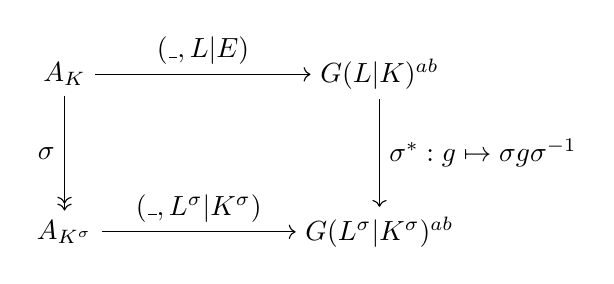
\begin{tikzpicture}[scale =1]
\node (D1) at (0,2)  {$A_K$};
\node (D3) at (4,2)  {$G(L|K)^{ab}$};
\node (D5) at (0,0)  {$A_{K^\sigma}$};
\node (D7) at (4,0)  {$G(L^\sigma|K^\sigma)^{ab}$};

\draw[->] (D1) -> (D3) node[midway, above]{$(\_, L|E)$};
\draw[->] (D5) -> (D7) node[midway, above]{$(\_, L^\sigma | K^\sigma)$};
\draw[->] (D3) -> (D7) node[midway, right]{$\sigma^* : g \mapsto \sigma g \sigma\i$};
\draw[->>] (D1) -> (D5) node[midway, left]{$\sigma$};
\end{tikzpicture}
\end{center}

\item[(A2)] Sei $K'|K$ eine endliche Erweiterung und setze $L' = K'L$. Dann kommutiert
\begin{center}
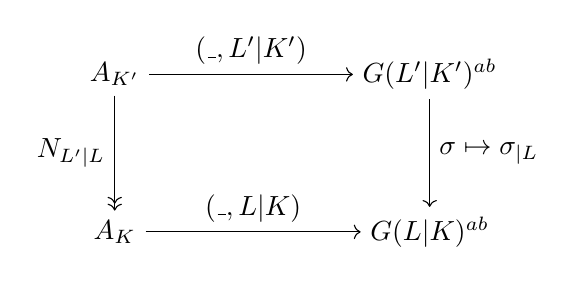
\begin{tikzpicture}[scale =1]
\node (D1) at (0,2)  {$A_{K'}$};
\node (D3) at (4,2)  {$G(L'|K')^{ab}$};
\node (D5) at (0,0)  {$A_{K}$};
\node (D7) at (4,0)  {$G(L|K)^{ab}$};

\draw[->] (D1) -> (D3) node[midway, above]{$(\_, L'|K')$};
\draw[->] (D5) -> (D7) node[midway, above]{$(\_, L | K)$};
\draw[->] (D3) -> (D7) node[midway, right]{$\sigma \mapsto \sigma_{|L}$};
\draw[->>] (D1) -> (D5) node[midway, left]{$N_{L'|L}$};
\end{tikzpicture}
\end{center}

\item[(A3)] Liegen endliche Körpererweiterungen $L|K'|K$ vor, sodass $L$ und $K'$ galoissch über $K$ sind, so kommutiert
\begin{center}
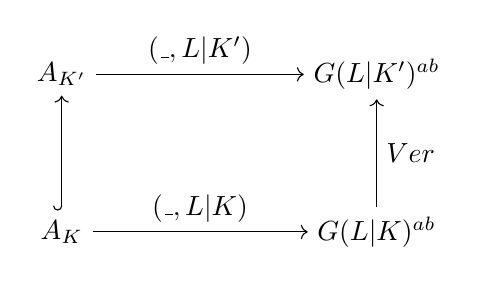
\begin{tikzpicture}[scale =1]
\node (D1) at (0,2)  {$A_{K'}$};
\node (D3) at (4,2)  {$G(L|K')^{ab}$};
\node (D5) at (0,0)  {$A_{K}$};
\node (D7) at (4,0)  {$G(L|K)^{ab}$};

\draw[->] (D1) -> (D3) node[midway, above]{$(\_, L|K')$};
\draw[->] (D5) -> (D7) node[midway, above]{$(\_, L | K)$};
\draw[->] (D7) -> (D3) node[midway, right]{$Ver$};
\draw[right hook->] (D5) -> (D1) node[midway, left]{};
\end{tikzpicture}
\end{center}
\end{itemize}

\section{Haupttheoreme der Klassenkörpertheorie}
\Def{Lokaler Körper}
Unter einem \df{lokalen Körper} verstehen wir $\R$ oder $\C$ oder einen vollständigen, diskret bewerteten Körper mit endlichem Restklassenkörper.

\Satz{Lokale Klassenkörpertheorie}
Sei $K$ ein lokaler Körper.
\begin{itemize}
\item Es existiert genau ein stetiger Gruppenhomomorphismus
\[ \phi_K : K^\times \Pfeil{} G_K^{ab} \]
der folgende Eigenschaften erfüllt:
\begin{itemize}
\item Für jede endliche, abelsche Erweiterung $L|K$ induziert $\phi_K$ einen Isomorphismus
\[ K^\times / N_{L|K} L^\times \Pfeil{\isom{}} G(L|K) \]
\item Ist $K\neq \R,\C$ und besitzt den endlichen Restklassenkörper $\kappa$, so kommutiert folgendes Diagramm
\begin{center}
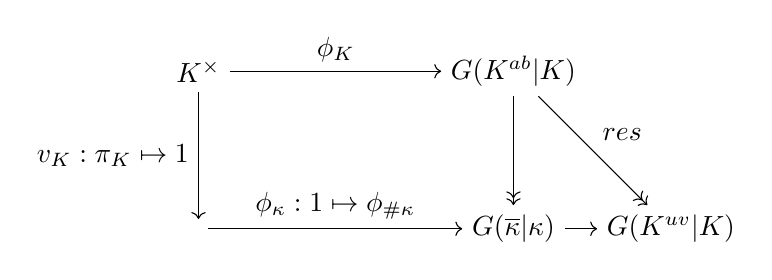
\begin{tikzpicture}[scale =1]
\node (D1) at (0,2)  {$K^\times$};
\node (D3) at (4,2)  {$G(K^{ab}|K)$};
\node (D5) at (0,0)  {$\Z$};
\node (D7) at (4,0)  {$G(\overline{\kappa}|\kappa)$};
\node (D9) at (6,0)  {$G(K^{uv}|K)$};

\draw[->] (D1) -> (D3) node[midway, above]{$\phi_K$};
\draw[->] (D5) -> (D7) node[midway, above]{$\phi_\kappa : 1 \mapsto \phi_{\#\kappa}$};
\draw[->>] (D3) -> (D7) node[midway, right]{};
\draw[->>] (D3) -> (D9) node[midway, above right]{$res$};
\draw[->] (D7) -> (D9) node[midway, above]{$\isom{}$};
\draw[->] (D1) -> (D5) node[midway, left]{$v_K:\pi_K\mapsto 1$};
\end{tikzpicture}
\end{center}
wobei $K^{ab}$ die maximale abelsche Erweiterung von $K$ und $K^{uv}$ ihre maximale unverzweigte Teilerweiterung ist.
\end{itemize}
\item Es ergeben sich folgende Korrespondenzen
\begin{center}
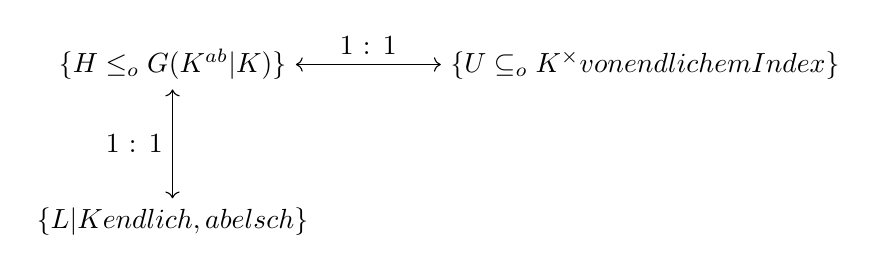
\begin{tikzpicture}[scale =2]
\node (D1) at (0,1)  {$\{H\leq_o G(K^{ab}|K)\}$};
\node (D3) at (3,1)  {$\{ U \subseteq_o K^\times \text{ von endlichem Index} \}$};
\node (D7) at (0,0)  {$\{ L |K \text{ endlich, abelsch} \}$};

\draw[<->] (D1) -> (D3) node[midway, above]{1 : 1};
\draw[<->] (D7) -> (D1) node[midway, left]{1 : 1};
%\draw [ultra thick, right hook->,    blue] (0,-1) -- (3,-1);
\end{tikzpicture}
\end{center}
\end{itemize}

\Def{Globale Körper}
Unter einem \df{globalen Körper} verstehen wir einen Zahl- bzw. Funktionenkörper.

\Satz{Globale Klassenkörpertheorie}
Sei $K$ ein globaler Körper, $C_K$ bezeichne seien Idelegruppe.
\begin{itemize}
\item Es existiert genau ein stetiger Gruppenhomomorphismus
\[ \phi_K : C_K \Pfeil{} G_K^{ab} \]
sodass für jede Stelle $v$ von $K$ folgendes Diagramm kommutiert
\begin{center}
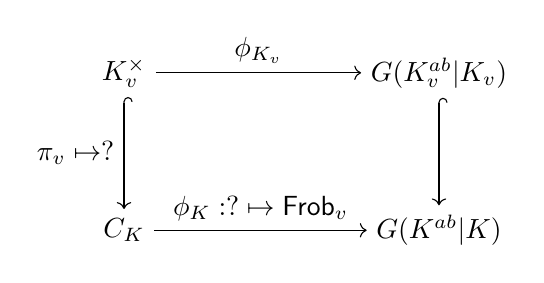
\begin{tikzpicture}[scale =1]
\node (D1) at (0,2)  {$K_v^\times$};
\node (D3) at (4,2)  {$G(K_v^{ab}|K_v)$};
\node (D5) at (0,0)  {$C_K$};
\node (D7) at (4,0)  {$G(K^{ab}|K)$};

\draw[->] (D1) -> (D3) node[midway, above]{$\phi_{K_v}$};
\draw[->] (D5) -> (D7) node[midway, above]{$\phi_K : ? \mapsto \Frob_v$};
\draw[right hook->] (D3) -> (D7) node[midway, right]{};
\draw[right hook->] (D1) -> (D5) node[midway, left]{$\pi_v \mapsto ?$};
\end{tikzpicture}
\end{center}
wobei $K_v$ die Komplettierung von $K$ bzgl. $v$ bezeichnet. 

\item Für jede endliche, abelsche Erweiterung $L|K$ induziert $\phi_K$ einen Isomorphismus
\[ C_K / N_{L|K} C_L \Pfeil{\isom{}} G(L|K) \]

\item Es ergeben sich folgende Korrespondenzen
\begin{center}
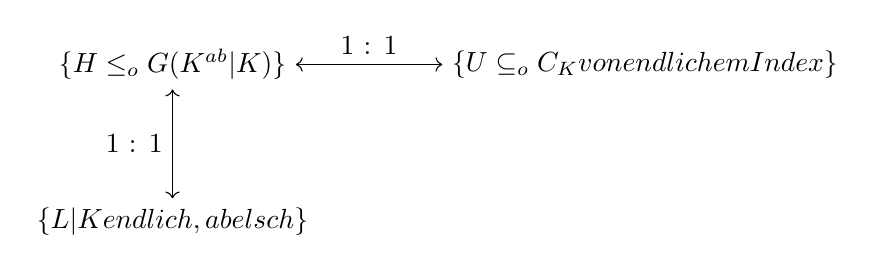
\begin{tikzpicture}[scale =2]
\node (D1) at (0,1)  {$\{H\leq_o G(K^{ab}|K)\}$};
\node (D3) at (3,1)  {$\{ U \subseteq_o C_K \text{ von endlichem Index} \}$};
\node (D7) at (0,0)  {$\{ L |K \text{ endlich, abelsch} \}$};

\draw[<->] (D1) -> (D3) node[midway, above]{1 : 1};
\draw[<->] (D7) -> (D1) node[midway, left]{1 : 1};
%\draw [ultra thick, right hook->,    blue] (0,-1) -- (3,-1);
\end{tikzpicture}
\end{center}
\end{itemize}

\section{Was besagt die Klassenkörpertheorie? Erste Folgerungen der Hauptresultate}
\Satz{}
Sei $L|K$ eine endliche, abelsche Erweiterung globaler Körper. $v$ sei eine Stelle von $K$, $\pi_v \in \O_{K_v} \subset K_v$ die zugehörige lokale Stelle. Definiere folgende Abbildung
\[ \Theta : K_v^\times \Inj{} C_K \Pfeil{} C_K/N_{L|K}C_L \]
Dann gilt
\begin{itemize}
\item $v$ zerlegt sich voll in $L$ $\Gdw{}$ $\Theta(K_v^\times) = \{1\}$
\item Ist $v$ endlich, so gilt
\[ v \text{ ist unverzweigt in }L\Gdw{} \Theta(\O_{K_v}^\times) = \{1\} \]
\item Sei $v$ endlich und unverzweigt in $L$. Dann liegt folgende Isomorphie vor
\begin{align*}
C_K / N_{L|K}C_L &\Pfeil{} G(L|K)\\
\Theta(\pi_v) & \longmapsto \Frob_v
\end{align*}
\end{itemize}

\chapter{Adele, Idele und Verallgemeinerte Idealklassengruppen}
\section{Eingeschränkte Produkte}
\Bem{}
Ab sofort heißt ein topologischer Raum \textit{kompakt}, falls er \textit{quasikompakt} und \textit{hausdorffsch} ist.\\
Ein Raum heißt ferner ab jetzt \textit{lokal kompakt}, falls er \textit{hausdorffsch} und \textit{lokal quasikompakt} ist.

\Def{Eingeschränkte Produkte}
Sei $I$ eine Indexmenge, $(G_i)_{i\in I}$ eine Familie lokal kompakter, abelscher Gruppen und $(U_i)_{i\in I}$ eine Familie jeweils kompakter, offener Untergruppen.\\
Definiere das \df{restringierte Produkt} bzw. \df{eingeschränkte Produkt} von $(G_i)_i$ bzgl. $(U_i)_i$ durch
\[ \prod_{i\in I}'G_i := \set{(x_i)_i \in \prod_{i\in I}G_i}{ x_i \in U_i \text{ ffa } i \in I } \]
Definiere für eine endliche Menge $J \subset I$
\[ G_J := \prod_{i \in J}G_i \times \prod_{i \in I\setminus J} G_i \]
Dann gilt
\[ \prod_{i\in I}'G_i = \bigcup_{J \text{ endlich}}G_J  \]
Jedes $G_J$ trägt die Produkttopologie und ist lokal kompakt; das restringierte Produkt $\prod_{i\in I}'G_i$ wird nun mit der dadurch induzierten Kolimestopologie versehen. Dadurch ist $\prod_{i\in I}'G_i$ ebenfalls lokal kompakt und für jedes $V \subset \prod_{i\in I}'G_i$ gilt insbesondere
\[ V \subset_o G \Gdw{} V\cap G_J \subset_o G_J \text{ für alle }J \text{ endlich} \]
Die Menge
\[ \set{ \prod_{i \in J}O_i \times \prod_{i \in I\setminus J}U_i }{J \subset I \text{ endlich und } 1 \in O_i \subset_o G_i} \]
bilde eine Umgebungsbasis der Eins in $\prod_{i\in I}'G_i$.\\
Ferner wird folgende universelle Abbildungseigenschaft für jede hausdorffsche, abelsche Gruppe $Z$ erfüllt
\[ \Hom{cts}{\prod_{i\in I}'G_i}{Z} = \set{(f_i)_i \in \prod_{i \in I} \Hom{cts}{G_i}{Z} }{ \text{ffa } i \in I \text{ ist } f_i(U_i) \text{ in jedem }1 \in U\subset_o Z \text{ enthalten} } \]


\section{Adele und Idele}
\Def{Adelering und Idelering}
Sei $K$ ein globaler Körper, $S$ die Menge aller Stellen von $K$. Definiere den \df{Adelering} von $K$ durch das restringierte Produkt
\[ \A_K := \prod'_{v\in S} K_v \text{ bzgl. } (\O_v)_{v\in S} \]
und die \df{Idelegruppe} durch
\[ \A_K^\times := \prod'_{v\in S}K_v^\times \text{ bzgl. } (\O_v^\times)_{v\in S} \]

\Bem{}
\[(\A_K)^\times = \A_K^\times \]
\Def{Hauptadele und Hauptidele}
Es liegen folgende Homomorphismen vor
\begin{align*}
K & \Inj{} \A_K && K^\times \Inj{} \A_K^\times\\
a & \longmapsto (a)_v && a\longmapsto (a)_v
\end{align*}
Die Bilder dieser Inklusionen nennen wir \df{Hauptadele} bzw. \df{Hauptidele}.\\
Die \df{Idele-Klassengruppe} ist definiert durch
\[ C_K := \A_K^\times / K^\times \]
Ferner liegt folgender stetiger multiplikativer Monoid-Homomorphismus vor
\begin{align*}
\bet{\cdot} : \A_K &\Pfeil{} \R_{\geq 0}\\
(a_v)_v & \longmapsto \bet{a} := \prod_{v}\bet{a}_v
\end{align*}

\Satz{Produktformel}
Sei $K$ global, dann gilt für alle $a \in K^\times$
\[ \bet{a} = 1 \]

\Satz{}
Sei $K$ global.
\begin{itemize}
\item $K$ liegt in $\A_K$ diskret und $\A_K/K$ ist kompakt.
\item Definiere
\[ \A_K^1 := \set{a\in\A_K^\times}{ \bet{a} = 1 } \]
$K^\times$ liegt in $\A_K^1$ diskret und $C^1_K:= \A_K^1/K^\times$ ist kompakt.
\end{itemize}

\Bem{}
$C_K = \A_K^\times/K^\times$ ist im Allgemeinem nicht kompakt.

\Bem{Idealklassengruppe}
Sei $K$ ein Zahlkörper, $\I$ bezeichne die Menge der gebrochenen Ideale von $K$, $\P$ die Menge der gebrochenen Hauptideale.\\
Die \df{Idealklassengruppe} ist definiert durch
\[Cl(K) = \I/\P \]
Bezeichnet $S_f$ die Menge der endlichen Stellen von $K$ und $S_\infty$ die Menge der unendlichen Stellen von $K$, so definiere
\[ \U := \prod_{v\in S_\infty}K_v^\times \times \prod_{v\in S_f} \O_v^\times \subset \A_K^\times \]
Es gilt
\[ \A_K^\times / \U \isom{} \bigoplus_{v\in S_f} K_v^\times / \O_v^\times \isom{} \I  \]
Definiert man ferner $\overline{\U} := K^\times\cdot\U/K^\times$, so gilt
\[ C_K / \overline{\U} \isom{} Cl(K) \]

\Def{Verallgemeinerte Idealklassengruppe}
Sei $K$ ein Zahlkörper.\\
Definiere für ein Ideal $0\neq \af \subset \O_K$
\[ \U(\af) := \prod_{v\in S}U_v(\af) \subset \U \]
wobei
\[ U_v(\af) := \left\lbrace
\begin{aligned}
\{x \in \O_{K_v}~|~x \equiv 1 \mod{\af\O_{K_v}}\} = 1 + \mf_v^{n_v(\af)} = 1 + \af \O_{K_v} && v \in S_f\\
K_v^\times && v \text{ komplex}\\
\R_{>0} \cap K^\times_v && v \text{ reell}
\end{aligned}
\right. \]
Die \df{verallgemeinerte Idealklassengruppe} ist definiert durch
\[Cl(K, \af) = C_K / \overline{\U(\af)} \]
Es gilt für Ideale $\af,\bf$
\[ \af \leq \bf \Gdw{} \U(\af) \leq \U(\bf) \Gdw{} Cl(K,\af) \surj{} Cl(K,\bf) \]
und
\[ Cl(K,\O_K) = Cl(K) \]

\Bem{Alternative Beschreibung der Idealklassengruppe}
Sei $K$ ein Zahlkörper, $0\neq \af \subset \O_K$ ein Ideal.\\
Es sei
\[ S(\af) := \set{v \in S_f}{n_v(\af) \neq 0} \]
Definiere für ein Ideal $0\neq \af \subset \O_K$ die Gruppe der zu $\af$ teilerfremden gebrochenen Ideale
\[ \I(\af) := \set{\bf\i \cf}{\bf,\cf \trianglelefteq \O_K \text{ teilerfremd zu } \af} \isom{} \bigoplus_{v\in S_f \setminus S(\af)}\Z \]
und die Gruppe der $\af$ teilerfremden gebrochenen Hauptideale
\[ \P(\af) := \set{(\alpha) \in K^\times}{\alpha \text{ ist lokal positiv und }\forall v \in S(\af): \alpha \in 1 + \af\O_{K_v}}  \]

\Bem{}
Im Allgemeinem gilt
\[ \P(\af) \subsetneq \P \cap \I(\af) \]
In jedem Fall gilt wegen dem Approximationsatz
\[ \I(\af) / \P \cap \I(\af) = \I / \P = Cl(K) \]

\Satz{}
Sei $K$ ein Zahlkörper, $0\neq \af \subset \O_K$ ein Ideal.\\
Setze
\[ S:= S_\infty \cup S(\af) \]
Beachte, dass für $v \notin S$ $U_v(\af) = \O_{K_v}^\times$ gilt. Wir erklären folgenden Homomorphismus
\begin{align*}
\phi : \I(\af) \isom{} \bigoplus_{v\notin S} \Z \isom{} \bigoplus_{v\notin S} K_v^\times / U_v(\af) \subset \A_K^\times / \U(\af) \surj{} C_K / \overline{\U(\af)} = Cl(K,\af)  
\end{align*}
Es gilt
\begin{itemize}
\item $\phi$ induziert einen Isomorphismus
\[ \phi : \I(\af) / \P(\af) \Pfeil{} Cl(K,\af) \]
\item Es liegt folgende kurze exakte Sequenz vor
\[ 1 \Pfeil{} \klam{ \bigoplus_{v \text{ reell}} \R^\times / \R_{>0} \oplus (\O_K / \af)^\times } / \O_K^\times \Pfeil{} Cl(K,\af) \Pfeil{} Cl(K) \Pfeil{} 1 \]
Insbesondere ist $Cl(K,\af)$ endlich.
\end{itemize}

\Satz{Approximationssatz}
Sei $K$ ein Zahlkörper, $S$ eine endliche Stellenmenge. Für jedes $v \in S$ sei ein $x_v \in K$ vorgegeben. Dann existiert für jedes $\epsilon >0$ ein $x \in K$, sodass für alle $v \in S$ gilt
\[ \bet{x-x_v}_v < \epsilon \]

\Def{}
Sei $K$ ein Zahlkörper, $0\neq \af \subset \O_K$ ein Ideal, $S = S_\infty \cup S(\af)$.\\
Definiere
\[ K_\af^\times := \Ker\klam{ K^\times \pfeil{} \bigoplus_{v\in S } K_v^\times / U_v(\af)}  \]
und
\[\O_{K,\af}^\times := K_\af^\times \cap \O_K^\times \]
Dann liegt folgende Isomorphie vor
\[ K_\af^\times / \O_{K,\af}^\times = \P(\af) \]
\end{document}